\section{Experimental Results and Discussions}\label{sec:results}
We demonstrate the effectiveness and scalability of random tree search using simulation.
We implemented the random tree search algorithm in C++\footnote{Our tools and data are open-source. Our repository can be accessed at \url{github.com/ahmadyan/Capacitated-Selfish-Replication-Game}} and ran our simulation on a Macbook pro laptop equipped with Core-i7 processor and 16GB of memory.

For case-studies, we use a randomly generated Erdos-Renyi graph $G(n,p)$, where $n$ is the number of players and $p$ is the probability of existence of an edge between two player. We ensured that the graph is connected. The CSR game is for $k$ number of resources in the graph $G$. We executed the random tree search algorithm to find the optimal allocation. The random tree would terminate when the cost function reaches it's maximum at $n\times k$. For each entry point, we repeat the experiments 100 times and reported the mean number of iterations and execition time. To ensure correctness, we checked the number of unsaturated neighborhoods in the graph $G$ to be zero at termination.


% two types of results:
% 1. Showing algorithm w.r.t. Number of iterations--> should be linear
% 2. Algorithm w.r.t. its runtime --> O(n^2)

\paragraph{Effects of player size on search}
Figure~\ref{fig:result1} shows the result of our algorithm for different games with different number of players. We generated a game graph $G(n, 0.05)$ with $k=5$ resources. As we increased the number of players, the optimal allocation became harder to locate, but the random tree algorithm quickly found the optimal allocation even for a game with 100 players. When we increased the number of players beyound 100, the search actually became easier. Because in Erdos graph with $p=0.05$, after 100 player, every player is connected to an expected number of $5$ players or more. Since we only have 5 resources in that game, there are many equilibrium points in the game. The random tree algoritm converged almost instantly from 200 to up-to 1000 players. Figure~\ref{fig:result2} shows the simulation time, in second, required for finding the optimal allocation. Althought the worst-case execution time of our algorithm is $O(n\times(n+e)\times b\log^2(b))$, in practice the actual simulation time is corrolated linearly with the number of iterations in our implementation.


\begin{figure}[htb]
\begin{center}
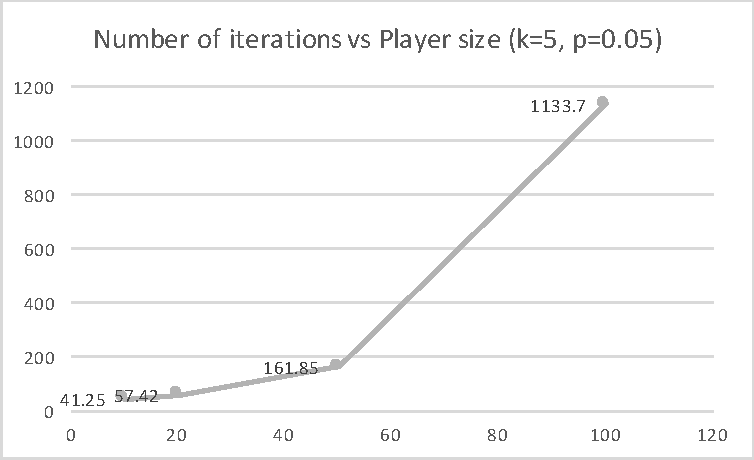
\includegraphics[width=.4\textwidth]{result-1}
\end{center}
\caption{The random tree search algorithm quickly found the opimal allocation for large scale graphs. As we increased the number of players, the number of iterations required for finding the optimal allocation also increased.}
\label{fig:result1}
\end{figure}

\begin{figure}[htb]
\begin{center}
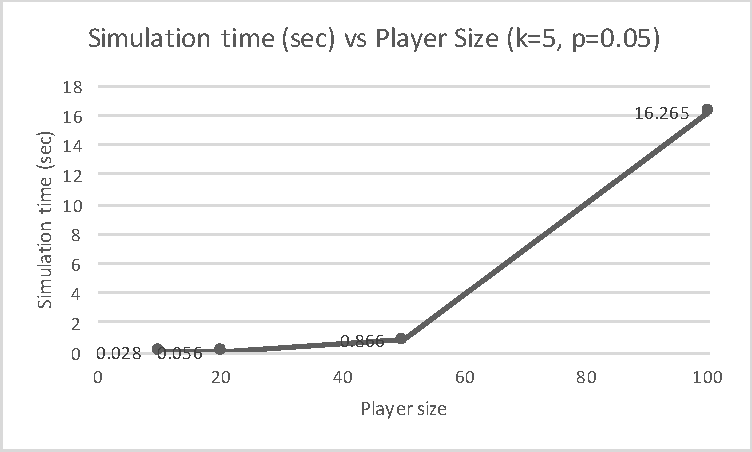
\includegraphics[width=.4\textwidth]{result-2}
\end{center}
\caption{As we increased the number of players, the simulation time required for finding the optimal allocation also increased. The simulation time was linearly corrolated with number of iterations.}
\label{fig:result2}
\end{figure}


%non-trivila result No.1
%when we increase the graph size for a fixed p, at the begining the problem gets harder and harder, but after a threshold point (n\p) the problem becomes a lot easier

\paragraph{Effects of graph sparsity on search}
The worst-case game occured where $n\times p == k$, where $n$ is the number of players, $k$ is number of resources and $p$ is probability of existence of an edge between two player. The expected number of edges between two player is $n\times p$. When the expected number of edges is far smaller than the number of resources, the radius of each player substantially increases. However the random tree has to make a fewer choices to satisfy players. As a result, the random tree search has to explore more space but the search will be easier. This can be seen in Figure~\ref{fig:result3}. On the other hand, when $n\times p >> k$, the search also becomes easier because every player is connected to many more players. As a result, the number of optimal allocations in the game increases and they become easier to find. In general, when the graph is too sparse the search was efficient. On the other hand, when the graph was too dense, there were multiple optimal solutions.


\begin{figure}[htb]
\begin{center}
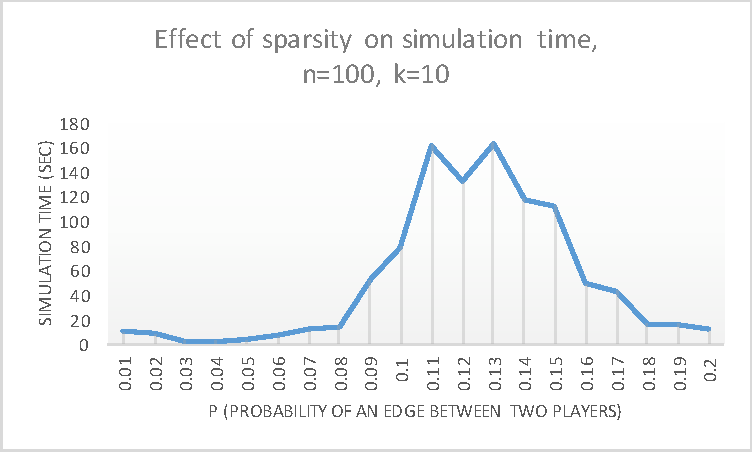
\includegraphics[width=.4\textwidth]{result-3}
\end{center}
\caption{When the graph was very sparse or very dense, the random tree quickly searched the state space and found the optimal allocation. However when the number of resources is roughtly $p\times n$, the search becames more complicated. The random tree stil quickly found the optimal allocation in less 4500 iterations on average. }
\label{fig:result3}
\end{figure}

\begin{figure}[htb]
\begin{center}
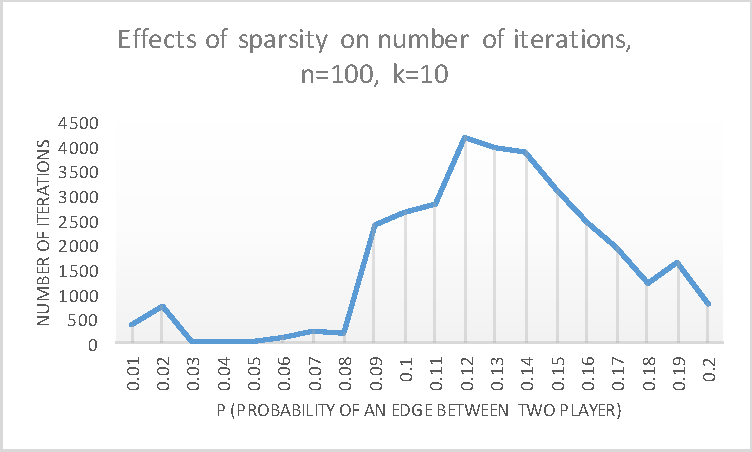
\includegraphics[width=.4\textwidth]{result-4}
\end{center}
\caption{the runtime for the random tree algorithm is linearly corrolated with the number of iterations. When the graph was very sparse or very dense, the random tree quickly searched the state space and found the optimal allocation. However when the number of resources is roughtly $p\times n$, the search becames more complicated. The random tree stil quickly found the optimal allocation in less than 3 minutes.}
\label{fig:result4}
\end{figure}

In order to understand the effect of resource size on the search algorithm complexity, we removed the dependency on the variable $p$ (probability of an edge between two players) from the Erdos Graph. Instead we used a randomly generated graph $K(n, e)$, where $n$ is the number of players in the graph and $e$ is the expected number of edges between two players. For each player $i$, we added $e$ edges between player $i$ and randomly chosen player $j$. We ensured that the graph was connected. Figure~\ref{fig:result_time_resources} shows the simulation time required for finding the optimal allocation for different random grpahs of 100 players versus for different resource sizes. We sat the number of expected edges equal as the number of resources in the game, because we saw eariler that would result in the worst-case execution of the algorithm. When the number of resource sizes is small, say 2 or 3, the random tree algorithm quickly converges toward the optimal allocation because the search space is very small. However, as the number of resources in the game increases, the search becomes harder. As shown in Figure~\ref{fig:result_time_resources} The runtime of the algorithm is linearly increases as the number of resources in the game increases.

\begin{figure}[htb]
\begin{center}
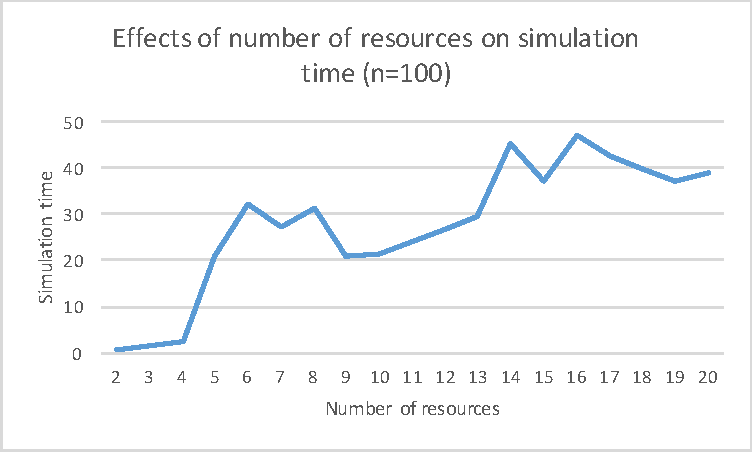
\includegraphics[width=.4\textwidth]{result-time-resources}
\end{center}
\caption{The runtime of the random tree algorithm for different resource sizes.}
\label{fig:result_time_resources}
\end{figure}
